
\section{Organization}
\subsection{Syllabus}
\frame{\frametitle{Main textbooks}
  \begin{itemize}
  \item<1-> Chierchia \& McConnell-Ginet, \textit{Meaning and Grammar}
  \item<2-> Partee, ter Meulen \& Wall, \emph{Mathematical Methods in Linguistics}
  \item<3-> Blackburn, Bos \& Striegnitz, \emph{Learn Prolog now!}
  \item<4-> Blackburn \& Bos, \emph{Computational Semantics for Natural Language}
  \end{itemize}
}

\frame{\frametitle{Further reading}
  \begin{itemize}
  \item<1-> Bucher, \emph{Einf\"uhrung in die angewandte Logik}
  \item<2-> Sag, Wasow \& Bender, \emph{Syntactic Theory}
  \item<3-> Dowty, \emph{Tense, Time Adverbs, and Compositional Semantic Theory}
  \item<4-> Partee, \emph{Noun Phrase Interpretation and Type-shifting Principles}
  \item<5-> Copestake, Flickinger \& Sag \emph{Minimal Recursion Semantics}
  \end{itemize}
}

\subsection{Course Structure}
\frame {
  \frametitle{The three sessions}
  \begin{itemize}
  \item<1-> Formal Semantics, 90 min. on Wednesday
  \item<2-> PROLOG, 30 min. on Wednesday
  \item<3-> Tutorial, 90 min. on Friday
  \item<4-> Summer course (implementation), 1 week
  \end{itemize}
}

\frame{ \frametitle{The first weeks: Preliminaries (subject to changes)}
\begin{center}\begin{tabular}{lp{7cm}}
  Session 1 &  Introduction to Referential Semantics \\
            &  \textcolor[rgb]{0.50,0.50,0.50}{(CM chap. 1 \& 2)} \\
  Session 2 &  Set theory, ordering theory, statement logic\\
   & \textcolor[rgb]{0.50,0.50,0.50}{(PMW chap. 1 - 6)} \\
  Session 3 &  Predicate calculi \textcolor[rgb]{0.50,0.50,0.50}{(PMW chap. 7 \& 8)}\\
\end{tabular}\end{center}
}

\frame{ \frametitle{The middle weeks: First steps (subject to changes)}
\begin{center}\begin{tabular}{lp{7cm}}
  Session 4 &  Quantification and model theory\\
   & \textcolor[rgb]{0.50,0.50,0.50}{(CM chap. 3)}\\
  Session 5 &  Quantification in English \textcolor[rgb]{0.50,0.50,0.50}{(CM chap. 3)}\\
  Session 6 &  Intensionality \textcolor[rgb]{0.50,0.50,0.50}{(CM chap. 5)}\\
  Session 7 &  Tense, modals, complementizers\\
            &  \textcolor[rgb]{0.50,0.50,0.50}{(CM chap. 5)}\\
  Session 8 &  $\lambda$ \textcolor[rgb]{0.50,0.50,0.50}{(CM chap. 7)}\\
\end{tabular}\end{center}
}

\frame{ \frametitle{The final weeks: Advanced topics (subject to changes)}
\begin{center}\begin{tabular}{lp{7cm}}
  Session 9 &  Word meaning \textcolor[rgb]{0.50,0.50,0.50}{(CM chap. 8)}\\
  Session 10 &  Generalized quantifiers  \textcolor[rgb]{0.50,0.50,0.50}{(CM chap. 7)}\\
  Session 11 &  Type shifting \textcolor[rgb]{0.50,0.50,0.50}{(Partee)}\\
  Session 12 &  Underspecified scope \textcolor[rgb]{0.50,0.50,0.50}{(Copestake \emph{et al.})}\\
  Session 13 & Backup session \\
  Session 14 &  \textcolor[rgb]{1.00,0.00,0.00}{Final test on 2004-07-13}\\
\end{tabular}\end{center}
}

\subsection{Our subject}

\frame{ \frametitle{What \emph{meaning} could mean}
  \begin{itemize}
  \item<1-> The meaning of an expression is the idea conveyed by it.
  \item<2-> \ldots is the mental image it creates.
  \item<3-> \ldots is what a speaker wants to achieve by uttering it.
  \item<4-> \ldots is the set of objects to which it refers (for example in the case of nouns).
  \end{itemize}
}

\frame{ \frametitle{What the study of meaning could be}
\begin{itemize}
  \item<1-> The study of the intellectual concepts perceivable in the world.
  \item<2-> \ldots of how the brain processes expressions, relates it to (fields of) cognitive 
  concepts.
  \item<3-> \ldots of how a discourse of planful and intelligent agents (humans) is structured.
  \item<4-> \textcolor[rgb]{0.00,0.00,1.00}{\ldots of the correspondences between expressions and objects; and of how expressions 
  are combined to be used productively.}
\end{itemize}
}

\frame{ \frametitle{What this class is about}
  \begin{itemize}
  \item<1-> Which objects do words refer to?
  \item<2-> What makes sentences true?
  \item<3-> How is the informational value of sentences related to their logical structure?
  \item<4-> How can sentences be unambiguously interpreted?
  \end{itemize}
}

\frame{ \frametitle{What this class is \textcolor[rgb]{1.00,0.00,0.00}{not} about}
  \begin{itemize}
    \item<1-> what words mean,
    \item<2-> how the brain works with sentences,
    \item<3-> the structure of discourse (at least not much).
  \end{itemize}
}

\section{Linguistic theories}
\subsection{Semiotics}
\frame{\frametitle{The theory of signs: a triangle}
  \begin{center}
  \begin{bundle}
  {forms:}
    \chunk{objects}
    \chunk{mental images}
  \end{bundle}
  \end{center}
}

\subsection{Generative Grammar}
\frame{\frametitle{Semantics in the Chomskian T-model} 
\begin{center}
  \includegraphics[scale=0.4]{\GRAPHPATH/tmodel.ps}
\end{center}
}

\subsection{Levels of representation}
\frame{\frametitle{LF is just the logical \textcolor[rgb]{1.00,0.00,0.00}{form}}
 \begin{itemize}
   \item<1-> No interpretation proper at LF.
   \item<2-> Movement transformations after the sentence has been uttered.
   \item<3-> At the LF level, sentences have a form compatible to their logic.
   \item<4-> Why? Syntax itself is often inadequate to express all alternatives of a sentence's logical representation.
 \end{itemize}
}

\section{A referential framework}

\frame{\frametitle{Some properties of language}
 \begin{itemize}
   \item<1-> aboutness
   \item<2-> referential nature
   \item<3-> informative
   \item<4-> objectiveness (of content)
   \item<5-> \textcolor[rgb]{0.00,0.00,1.00}{But which linguistic elements refer to what?}
 \end{itemize}
}

\subsection{The simple case}

\frame{\frametitle{Names}
\begin{center}
\begin{tabular}{ccc}
 an individual name & $\longrightarrow$ & one object in the world \\
 \node{a-1}{\emph{Harald Schmidt}} &  & \node{a-2}{\includegraphics[scale=0.3]{\GRAPHPATH/hs.ps}} \\
\end{tabular}
\end{center}
  \anodeconnect[r]{a-1}[l]{a-2}
}

\frame{\frametitle{Common nouns}
\begin{center}
\begin{tabular}{ccc}
 a common noun & $\longrightarrow$ & lots of objects \\
 \node{b-1}{\emph{soldier}} &  & \node{b-2}{\includegraphics[scale=0.3]{\GRAPHPATH/soldiers.ps}} \\
                 &  & \\
                 &            & \node{b-3}{etc.} \\
\end{tabular}
\end{center}
  \anodeconnect[r]{b-1}[l]{b-2}
  \anodeconnect[r]{b-1}[l]{b-3}
}

\frame{\frametitle{Adjectives}
\begin{center}
\begin{tabular}{ccc}
 an adjective & $\longrightarrow$ & lots of different objects of different kinds\\
 \node{c-1}{\emph{is human}} &  & \node{c-2}{\includegraphics[scale=0.3]{\GRAPHPATH/hs.ps}} \\
                 &  & \\
                 &  & \node{c-3}{\includegraphics[scale=0.3]{\GRAPHPATH/soldiers.ps}} \\
                 &            & \node{c-4}{\includegraphics[scale=0.3]{\GRAPHPATH/soccer.ps}} \\
\end{tabular}
\end{center}
  \anodeconnect[r]{c-1}[l]{c-2}
  \anodeconnect[r]{c-1}[l]{c-3}
  \anodeconnect[r]{c-1}[l]{c-4}
}

\subsection{Complex cases}

\frame{\frametitle{Sentences} 
\begin{center}
\begin{tabular}{p{3cm}cc}
 a sentence & $\longrightarrow$ & a situation, a fact, \dots\\
 \emph{\node{d-1}{A humming bird} is hovering over a red flower\node{d-1b}{.}} &  & \node{d-2}{\includegraphics[scale=0.3]{\GRAPHPATH/hummingbird.ps}} \\
  & \node{d-3}{\textcolor{red}{not at all}} & \node{d-4}{\includegraphics[scale=0.3]{\GRAPHPATH/hs.ps}} \\
  & \node{d-5}{\textcolor{red}{(object type mismatch)}} & \\
\end{tabular}
\end{center}
  \anodeconnect[t]{d-1}[l]{d-2}
  \nodeconnect[r]{d-1b}[l]{d-3}
  \anodeconnect[r]{d-3}[l]{d-4}
}

\frame{\frametitle{Frege's Principle: Meaning is compositional}
 \begin{itemize}
   \item<1-> \emph{A humming bird} $\longrightarrow$ one of many individuals 
   \item<2-> \emph{is hovering}  $\longrightarrow$ a property of that individual
   \item<3-> \emph{over} $\longrightarrow$ a relation between individuals
   \item<4-> \emph{a red} $\longrightarrow$ a property of another individual
   \item<5-> \emph{flower} $\longrightarrow$ the other one of many individuals
   \item<6-> \textcolor{red}{\emph{is hovering over a red flower} $\longrightarrow$ a complex property.}
 \end{itemize}
}

\frame{\frametitle{Recursion: infinite use of finite means}
 \begin{itemize}
   \item<1-> Frege's principle is indispensable!
   \item<2-> \emph{Harald Schmidt is \textcolor{blue}{human}.}
   \item<3-> \emph{Harald Schmidt is \textcolor{blue}{human} and \textcolor{blue}{tall}.}
   \item<4-> \emph{Harald Schmidt is \textcolor{blue}{human} and \textcolor{blue}{tall} and \textcolor{blue}{male}.}
   \item<5-> \emph{Harald Schmidt is \textcolor{blue}{human} and \textcolor{blue}{tall} and \textcolor{blue}{male} and \textcolor{blue}{not blue}.}
   \item<6-> \emph{Harald Schmidt is \textcolor{blue}{human} and \textcolor{blue}{tall} and \textcolor{blue}{male} and \textcolor{blue}{not blue} and \textcolor{blue}{grumpy in the morning}...}
 \end{itemize}
}

\section{Some fundamental semantic notions}
\frame{\frametitle{Basic semantics judgements}
 \begin{itemize}
   \item<1-> entailment
   \item<2-> presupposition
   \item<3-> ambiguity
   \item<4-> synonymy
 \end{itemize}
}

\subsection{Entailment}
\frame{\frametitle{Entailment: pure logic}
 \begin{itemize}
   \item<1-> A: \emph{This is electronic.}
   \item<2-> B: \emph{This is a presentation.}
   \item<3-> \textcolor{blue}{C follows logically: \emph{This is an electronic presentation.}}
   \item<4-> \textcolor{blue}{$A, B\vdash C$}
   \item<5-> \textcolor{red}{$A\not\vdash C$}
   \item<6-> \textcolor{red}{$B\not\vdash C$}
 \end{itemize}
}

\frame{\frametitle{Entailment: pure logic, formally}
 \begin{itemize}
   \item<1-> D: \emph{Harald Schmidt is human.}
   \item<2-> \textcolor{blue}{E follows logically: \emph{Something is human.}}
   \item<3-> \textcolor{blue}{$D\vdash E$}
   \item<4-> \textcolor{blue}{$D\wedge D$ follows logically: \emph{Harald Schmidt is human and Harald Schmidt is human.}}
   \item<5-> \textcolor{blue}{$D \vdash D\wedge D$}
 \end{itemize}
}

\frame{\frametitle{Tests: X entails Y if...}
 \begin{itemize}
   \item<1->When X is true, Y is true.
   \item<2->A situation described by Y is also described by X.
   \item<3->The information given by Y is fully contained in the information given by X.
   \item<4->One cannot say X is true and Y is false.
\end{itemize}
}

\frame{\frametitle{Entailments?}
 \begin{itemize}\small
   \item<2->\emph{Harald Schmidt is a talkmaster. $\rightarrow$ Harald Schmidt is human.}
   \item<3->\emph{Harald Schmidt is tall. $\rightarrow$ Someone is tall.}
   \item<4->\emph{Some humans are tall. $\rightarrow$ Harald Schmidt is tall.}
   \item<5->\emph{I have listened to Paul Kalkbrenner's new 12'' on bpitchcontrol. $\rightarrow$ Paul Kalkbrenner has released a 12'' on bpitchcontrol.}
   \item<6->\emph{After I had a Beck's, I installed RedHat on my PC. $\rightarrow$ I had a Beck's.}
   \item<7->\emph{After the bootloader had failed to boot RedHat on my PC, I had another Beck's. $\rightarrow$ RedHat has never booted on my PC.}
   \item<8->\emph{My flatmate likes Beck's. $\rightarrow$ My flatmate hates beer.}
   \item<9->\emph{Harald Schmidt cancelled his show. $\rightarrow$ Harald Schmidt's show was cancelled.}
\end{itemize}
}

\subsection{Presupposition}
\frame{\frametitle{Presuppostion: the background}
 \begin{itemize}
   \item<1->A: \emph{Willy Brandt is the current chancelor of the FRG.}
   \item<2->B: \emph{If Willy Brandt is the current chancelor of the FRG, why doesn't he do something?}
   \item<3->C: \emph{Willy Brandt is not the current chancelor of the FRG.}
   \item<4->\textcolor{blue}{A and B presuppose D: \emph{Willy Brandt is alive.}, C doesn't.}
   \item<5->\textcolor{blue}{A, B, and C presuppose E: \emph{There is a chancelor of the FRG}.}
   \item<6->Note: A $\vdash$ D, A $\vdash$ E
   \item<7->But: \textcolor{red}{B $\not\vdash$ D, B $\not\vdash$ E, C $\not\vdash$ E}
\end{itemize}
}

\frame{\frametitle{Presuppostion: two tests}
 \begin{itemize}
   \item<1->Presuppositions are triggered by all sorts of sentences (incl. negations, modals, conditionals, etc.).
   \item<2->Presuppositions can be negated while the sentence which presupposes them remains true. Entailments cannot be negated while keeping the entailing sentence true.
\end{itemize}
}

\subsection{Ambiguity, Synonymy, Vagueness, \ldots}
\frame{\frametitle{Ambiguity in syntax}
 \begin{itemize}
   \item<1-> \emph{She saw the man with a telescope.}
   \item<2-> {She [saw the man] with a telescope.}
   \item<3-> {She saw [the man with a telescope].}
 \end{itemize}
}

\frame{\frametitle{Ambiguity in semantics: scope}
 \begin{itemize}
   \item<1-> \emph{Everybody loves somebody.}
   \item<2-> Every person loves at least one other person.\\(Needn't be the same.)
   \item<3-> There is one person loved by everyone
 \end{itemize}
}

\frame{\frametitle{Synonymy} 
 \begin{itemize}
   \item<1-> Lexical synonymy: \emph{humming bird} $\stackrel{lex}{\equiv}$ \emph{colibri}
   \item<2-> Compositionally (\textbf{equivalence}): \emph{Mulder met his abducted sister after he broke into the secret army base.} $\equiv$ \emph{Before meeting his abducted sister, Mulder broke into the secret army base.}
   \item<3-> \textcolor{blue}{A $\equiv$ B iff A $\vdash$ B and B $\vdash$ A}
 \end{itemize}
}

\section{From reference to sense}
\subsection{Referential and non-referential NPs}
\frame{\frametitle{Noun-like expressions and complex NPs}
 \begin{itemize}
   \item<1-> I saw \textcolor{blue}{a man}.
   \item<2-> I saw \textcolor{blue}{the green wobbly thing crawling near}.
   \item<3-> I saw \textcolor{blue}{it}.
 \end{itemize}
}

\frame{\frametitle{Problems with referential NPs}
 \begin{itemize}
   \item<1-> \emph{\textcolor{blue}{The dark subatomic particles in the universe} have a total mass much larger than the visible subatomic particles.}
   \item<2-> \emph{\textcolor{blue}{Problems with referential semantic theories} don't concern \textcolor{blue}{Rumpletweezer}.}
   \item<3-> \textcolor{red}{and of course, vagueness (e.g., Sorites Paradox)}
 \end{itemize}
}

\frame{\frametitle{Problems with non-referential NPs}
 \begin{itemize}
   \item<1-> \emph{some guy}
	 \item<2-> \emph{not the faintest trace of blood}
	 \item<3-> \emph{any axiom of Zermelo-Fraenkel set theory}
 \end{itemize}
}

\subsection{A `reference' for complex terms?}
\frame{\frametitle{Beyond pointin-at-and-naming}
We need a logic to explain for effects like:\\

\bigskip
 \begin{tabular}{clr}
	&\textcolor{blue}{my humming bird's favorite flower} & is red \\
  $\vdash$&\textcolor{blue}{some flower} & is red \\
\end{tabular}
}

\subsection{Sentences refer to 0 and 1}
\frame{\frametitle{Some content-synonymous simple expressions}
\begin{itemize}
  \item<1-> a: \emph{colibri}
  \item<2-> b: \emph{humming bird}
  \item<3-> c: \emph{a brunette lady}
  \item<4-> d: \emph{a brown-haired dame}
  \item<5-> e: \emph{the primates}
  \item<6-> f: \emph{the apes and humans}
  \item<7-> \textcolor{blue}{a $\stackrel{lex}{\equiv}$ b, c $\stackrel{lex}{\equiv}$ d, e $\stackrel{lex}{\equiv}$ f}
\end{itemize}
}

\frame{\frametitle{Some content-synonymous complex expressions}
\begin{itemize}
  \item<1-> A: \emph{\textcolor{blue}{A colibri} is hovering over a red flower.}
  \item<2-> B: \emph{\textcolor{blue}{A humming bird} is hovering over a red flower.}
  \item<3-> C: \emph{Lauren Bacall was \textcolor{blue}{a brunette lady}}
  \item<4-> D: \emph{Lauren Bacall was \textcolor{blue}{a brown-haired dame}}
  \item<5-> E: \emph{\textcolor{blue}{Primates} are intelligent.}
  \item<6-> F: \emph{\textcolor{blue}{The apes and humans} are inteligent.}
  \item<7-> \textcolor{blue}{A $\equiv$ B, C $\equiv$ D, E $\equiv$ F}
\end{itemize}
}

\frame{\frametitle{Two axioms}
\begin{itemize}
\item<1-> \textcolor{blue}{Ax1}	Two expressions (e.g., NPs, sentences) that are synonymous have the same reference.
\item<2-> Formally: A $\equiv$ B then $\llbracket$A$\rrbracket$ = $\llbracket$B$\rrbracket$
\item<3-> Note: $\llbracket$A$\rrbracket$ is applicable to simplex and complex expressions A; it just produces the reference of A.
\item<3-> \textcolor{blue}{Ax2}	If we replace expression B within expression A with the synonymous expression C, then A does not change its reference.
\item<4-> Formally: If $\llbracket$B$\rrbracket$ = $\llbracket$C$\rrbracket$ then $\llbracket$[\Sub{A} B]$\rrbracket$ = $\llbracket$[\Sub{A} C]$\rrbracket$
\end{itemize}
}	

\frame{\frametitle{One common property of sentences: the truth value}
\begin{itemize}
  \item<1-> A: \emph{Lauren Bacall was a brunette lady.} (assumed to be true in the actual world)
  \item<2-> B: \emph{My cat sleeps quietly.} (assumed to be true in the actual world)
\end{itemize}
}

\frame{\frametitle{First conclusion}
\begin{itemize}
  \item <1-> $[\Sub{T} A]$ = \emph{The truth value of `Lauren Bacall was a brunette lady' is 1}.
  \item <2-> $[\Sub{T} B]$ = \emph{The truth value of `My cat sleeps quietly' is 1}.
  \item <3-> Such that \textcolor{blue}{A $\equiv [\Sub{T} A]$} and \textcolor{blue}{B $\equiv [\Sub{T} B]$}. \\ \footnotesize(Check: Whenever A is true, $[\Sub{T} A]$ is true and v.v.)
  \item <4-> So, by Ax1 \textcolor{blue}{$\llbracket$A$\rrbracket$ = $\llbracket [\Sub{T} A]\rrbracket$}\\
     and \textcolor{blue}{$\llbracket$B$\rrbracket$ = $\llbracket [\Sub{T} B]\rrbracket$}
\end{itemize}
}		

\frame{\frametitle{Second conclusion}
\begin{itemize}
  \item<1-> Check the denotations of the contained NPs:\\ \textcolor{blue}{$\llbracket$\emph{the truth value of A}$\rrbracket$ = $\llbracket$\emph{the truth value of B}$\rrbracket$ = 1}
  \item<2-> Such that by Ax2:\\ \textcolor{blue}{$\llbracket [\Sub{T} A]\rrbracket$ = $\llbracket [\Sub{T} B]\rrbracket$}
  \item<3-> \footnotesize{Why? Exchanging the referentially identical NPs `the truth value of A' and `the truth value of B' in the otherwise identical sentences `\_ is 1' forces us to conclude by Ax2 that also the whole sentences must have the same reference. Our book (CM) is a bit vague on that point.}
\end{itemize}
}		

\frame{\frametitle{Final conclusion}
\begin{center}
 \Large\textcolor{blue}{$\llbracket$A$\rrbracket$ = $\llbracket  [\Sub{T} A]\rrbracket$ = $\llbracket [\Sub{T} B]\rrbracket$ = $\llbracket$B$\rrbracket$ = 1}\\
 \medskip
 \textcolor{green}{Sentences denote truth values.}\\
 \medskip
\end{center}
}

\frame{\frametitle{Advantages of truth values}
\begin{itemize}
  \item<1-> indirect encoding of `richer' semantics (One must know the truth conditions of a sentence and the state of affairs to decide about the truth of a sentence.)
  \item<2-> a minimal common semantic property of sentences
  \item<3-> easily computable in a formal system (binary)
  \item<4-> their logic provides a basis for `richer' semantics (cf. second half of class)
\end{itemize}
}

\subsection{Sense and reference}
\frame{\frametitle{Frege also thought, reference couldn't be all}
\begin{center}
\begin{tabular}{|l|l|l|}
  \hline
  \textbf{Type} & \textbf{Reference} & \textbf{Sense} \\
  \hline
  \hline
  NP & individuals & individual concepts \\
      & \emph{Venus} & \\
  \hline
  VP & sets & property concepts \\
  & \emph{humming birds} & \\
  \hline
  S & 1 or 0 & thoughts \\
  & \emph{I like cats.} & \\
  \hline
\end{tabular}
\end{center}
}

\frame{\frametitle{Some terminology}
\begin{itemize}
  \item<1-> \emph{reference} = \emph{extension}	= what we're dealing with first
  \item<2-> \emph{sense} = \emph{intension} = what we will be dealing with later
  \item<3-> \emph{proposition} = the intensions of sentences as informational content: The `thought that S'.
\end{itemize}
}

\section{We're talking in fragments: F1}
\frame{\frametitle{Decomposing compositionality and composing truth}
\begin{itemize}
 \item<1-> How are sentences compositionally built up? 
 \item<2-> What do their parts denote?
 \item<3-> How does the denotation of the parts contribute to the whole.
 \item<4-> T-sentences: \textcolor{blue}{S of L is true in v iff p.}
 \item<5-> {\footnotesize \emph{S} a sentence, \emph{L} a language, \emph{v} a state of affairs, \emph{p} a statement of the truth conditions.}
\end{itemize}
}

\subsection{A syntax}

\frame{\frametitle{A phrase-structure grammar}
\begin{itemize}
 \item<1-> S $\rightarrow$ N VP
 \item<2-> S $\rightarrow$ S conj S	
 \item<3-> S $\rightarrow$	neg S
 \item<4-> VP $\rightarrow$ V\Sub{{i}}
 \item<5-> VP $\rightarrow$ V\Sub{t} N
\end{itemize}
}

\frame{\frametitle{A lexicon}
\begin{itemize}
 \item<1-> N $\rightarrow$ \emph{Herr Webelhuth, Frau Eckardt, the Turm-Mensa}
 \item<1-> V\Sub{{i}} $\rightarrow$ \emph{is relaxed, is creative, is stupid}
 \item<1-> V\Sub{t} $\rightarrow$ \emph{prefers}
 \item<1-> conj $\rightarrow$ \emph{and, or}
 \item<1-> neg $\rightarrow$ \emph{it is not the case that}
\end{itemize}
}

\subsection{The semantics: individuals, sets, functions, T-sentences}
\frame{\frametitle{Simple denotiations}
\begin{itemize}
  \item<1-> $\llbracket$Herr Webelhuth$\rrbracket$ = Herr Webelhuth
  \item<2-> $\llbracket$Frau Eckardt$\rrbracket$ = Frau Eckardt
  \item<3-> $\llbracket$the Turm-Mensa$\rrbracket$ = the Turm-Mensa
  \item<4-> $\llbracket$is relaxed$\rrbracket$ = \{x:x is relaxed\}
  \item<5-> $\llbracket$is creative$\rrbracket$ = \{x:x is creative\}
  \item<6-> $\llbracket$is stupid$\rrbracket$ = \{x:x is stupid\}
  \item<7-> $\llbracket$prefers$\rrbracket$ = \{$\langle$x,y$\rangle$: x prefers y\}
\end{itemize}
}

\frame{\frametitle{Some words don't really `denote', they act like functions}
\begin{itemize}
  \item<1-> $\dem{neg} = \left[
                         \begin{array}{l}
	                          1 \rightarrow 0\\
	                          0 \rightarrow 1
                         \end{array}
                         \right]$
  \item<2-> $\dem{and} = \left[
                         \begin{array}{l}
	                          \langle 1,1 \rangle \rightarrow 1\\
	                          \langle 1,0 \rangle \rightarrow 0\\
	                          \langle 0,1 \rangle \rightarrow 0\\
	                          \langle 0,0 \rangle \rightarrow 0
                         \end{array}
                         \right]$
  \item<3-> $\dem{or} = \left[
                         \begin{array}{l}
	                          \langle 1,1 \rangle \rightarrow 1\\
	                          \langle 1,0 \rangle \rightarrow 1\\
	                          \langle 0,1 \rangle \rightarrow 1\\
	                          \langle 0,0 \rangle \rightarrow 0
                         \end{array}
                         \right]$
  \end{itemize}
}

\frame{\frametitle{T-sentences: rule-to-rule}
\begin{itemize}
  \item<1-> \den{[\Sub{S}{ }N{ }VP]} = 1 iff \den{N} $\in$ \den{VP}, else 0
  \item<2-> \den{[\Sub{S} S1 conj S2]} = \den{conj} ($\langle$\den{S1},\den{S2}$\rangle$)
  \item<3-> \den{[\Sub{S} neg S]} = \den{neg} (\den{S})
  \item<4-> \den{[\Sub{VP} V\Sub{t} N]} = \{x: $\langle$x, \den{N} $\rangle$ $\in$ \den{V\Sub{t}}\}
  \item<5-> semantics for non-branching nodes: \textcolor{blue}{pass-up}
\end{itemize}
}

\subsection{Bottom-up evaluation}
\frame{\frametitle{A starting point for our computation}
\textcolor{blue}{\emph{Herr Webelhuth is relaxed.}}\\

\begin{itemize}
  \item<1-> Circumstances (Model): Herr Webelhuth is an element of the set of relaxed individuals.\\{}
  \item<2-> (1) The syntax is well-formed by S $\rightarrow$ N VP
  \item<3-> (2) for N: \den{Herr Webelhuth} = Herr Webelhuth
  \item<4-> (3) for VP: \den{is relaxed} = \{x: x is relaxed\}
  \item<5-> (4) for S: \den{[\Sub{S}{ }N{ }VP]} = 1 iff \den{N} $\in$ \den{VP}, else 0
\end{itemize}
}

\frame{\frametitle{A starting point for our computation}
The tree:\\

\begin{center}
 \begin{bundle}
   {1 since \den{Herr Webelhuth} $\in$ \den{is relaxed}}
     \chunk[N]{\den{Herr Webelhuth}}
     \chunk[VP]{\den{is relaxed}}
 \end{bundle}
\end{center}
}

\frame{\frametitle{We compute syntactic representations, not flat sentences}
\emph{\textcolor{blue}{(\Sub{S1} Frau Eckardt is creative)} and it is not the case that \textcolor{green}{(\Sub{S2} Herr Webehlhuth is relaxed)} and \textcolor{red}{(\Sub{S3} Frau Eckardt prefers the Turm-Mensa)}.}\\
\begin{center}
\begin{tabular}{cc}
 \begin{bundle}
   {S}\setlength\GapDepth{2ex}\setlength\GapWidth{1em}
   \chunk{\textcolor{blue}{S\Sub{1}}}
     \chunk{conj}
     \chunk{
             \begin{bundle}
               {S}
               \chunk{neg}
               \chunk{\begin{bundle}
                         {S}
                         \chunk{\textcolor{green}{S\Sub{2}}}
                         \chunk{conj}
                         \chunk{\textcolor{red}{S\Sub{3}}}
                       \end{bundle}
                     }
             \end{bundle}        
           }
 \end{bundle} &
 \begin{bundle}
   {S}\setlength\GapDepth{2ex}\setlength\GapWidth{1em}
     \chunk{\textcolor{blue}{S\Sub{1}}}
     \chunk{conj}
     \chunk{
             \begin{bundle}
               {S}
               \chunk{\begin{bundle}
                       {S}
                       \chunk{neg}
                       \chunk{\textcolor{green}{S\Sub{2}}}
                      \end{bundle}
                     }
               \chunk{conj}
               \chunk{\textcolor{red}{S\Sub{3}}}
             \end{bundle}        
           }
 \end{bundle}  \\
\end{tabular}
\end{center}
}

\frame{\frametitle{A starting point for our computation}
Circumstances: Herr Webelhuth is relaxed, Frau Eckardt is creative, and Frau Eckardt does not prefer the Turm-Mensa:\\

\begin{center}
\begin{tabular}{cc}
 \begin{bundle}
   {1}\setlength\GapDepth{2ex}\setlength\GapWidth{1em}
     \chunk{\textcolor{blue}{1}}
     \chunk{conj}
     \chunk{
             \begin{bundle}
               {1}
               \chunk{neg}
               \chunk{\begin{bundle}
                         {0}
                         \chunk{\textcolor{green}{1}}
                         \chunk{conj}
                         \chunk{\textcolor{red}{0}}
                       \end{bundle}
                     }
             \end{bundle}        
           }
 \end{bundle} &
 \begin{bundle}
   {0}\setlength\GapDepth{2ex}\setlength\GapWidth{1em}
     \chunk{\textcolor{blue}{1}}
     \chunk{conj}
     \chunk{
             \begin{bundle}
               {0}
               \chunk{\begin{bundle}
                       {0}
                       \chunk{neg}
                       \chunk{\textcolor{green}{1}}
                      \end{bundle}
                     }
               \chunk{conj}
               \chunk{\textcolor{red}{0}}
             \end{bundle}        
           }
 \end{bundle}  \\
\end{tabular}
\end{center}
}

